\documentclass[12pt]{article}
\usepackage{graphicx}
\usepackage[british,UKenglish,USenglish,english,american]{babel}
\usepackage{tocbibind}
\usepackage[toc,page]{appendix}

%--------------dodatkowe pakiety:-----------
\usepackage{mathtools}
\usepackage{amsfonts}
\usepackage{amsmath}
\usepackage{amsthm}
\usepackage{array}
% for code snippets:
\usepackage{listings}
% for plots:
\usepackage{pgfplots}
\pgfplotsset{width=11cm,compat=1.9}
%-------------------links------------------
\usepackage{hyperref}
\hypersetup{
    colorlinks=true,
    linkcolor=blue,
    filecolor=magenta,      
    urlcolor=cyan,
}
 
\urlstyle{same}
%------placing image caption at the bottom---------
\usepackage{floatrow}
%--------------allows pic alligning----------------
\usepackage[export]{adjustbox}
%-----------------------------------------------------
\begin{document}

\title{Introduction to CUDA and OpenCL}
\author{Ilona Tomkowicz, Zofia Wpisz swoje nazwisko}

\maketitle
\tableofcontents
\newpage
%--------------------------------------------------------------------

\section{Communication with GPU} \label{gpu_communication}

In order to check details about the GPU used by VM on labolatories (GeForce GTX 1060 6GB) we used a template project deviceQuery.

\subsection{How to establish connection with device} \label{ht_open_connection}
To etract information about the devices connected to host we use funcion
\begin{lstlisting}[language=C]
cudaGetDeviceCount(&deviceCount)
\end{lstlisting} cudaGetDeviceCount(\&deviceCount), which returnes the flag message and changed the passed argument according to the number of devices that were found. Setting onection is done by calling:
\begin{lstlisting}[language=C]
cudaSetDevice(dev_index);
\end{lstlisting}
Where dev\_index is the index of GPU found (for only 1 GPU it will be 0).

\subsection{How to fetch information about GPU} \label{fetch_info}
To fetch information about GPU, after completing steps in previous point, we can call:
\begin{lstlisting}[language=C]
cudaDeviceProp deviceProp;
cudaGetDeviceProperties(&deviceProp, dev_index).
\end{lstlisting}
to get information about device properties or 
\begin{lstlisting}[language=C]
cudaDriverGetVersion(&driverVersion);
cudaRuntimeGetVersion(&runtimeVersion);
\end{lstlisting}
to check driver and runtime version.
After that we can extract specific data like memory size, clock rate, etc using these functions parameters.

\section{Experiments with data size and grid layout}  \label{experients}
Experiments with performance were made using template vectorAdd. This template originally
\begin{itemize}
\item allocates memory in host and device,
\item copies the host input vectors A and B into device memory,
\item sets grid layout,
\item uses created kernel to make caculations,
\item copies the result back into host,
\item veifies if the result is correct
\item frees memory on both, device and host.
\end{itemize} 
Number of elements is changed for fixed gird layout and grid layout is changed for fixed number of elements.
\subsection{Computation time comparison}  \label{size_tests}

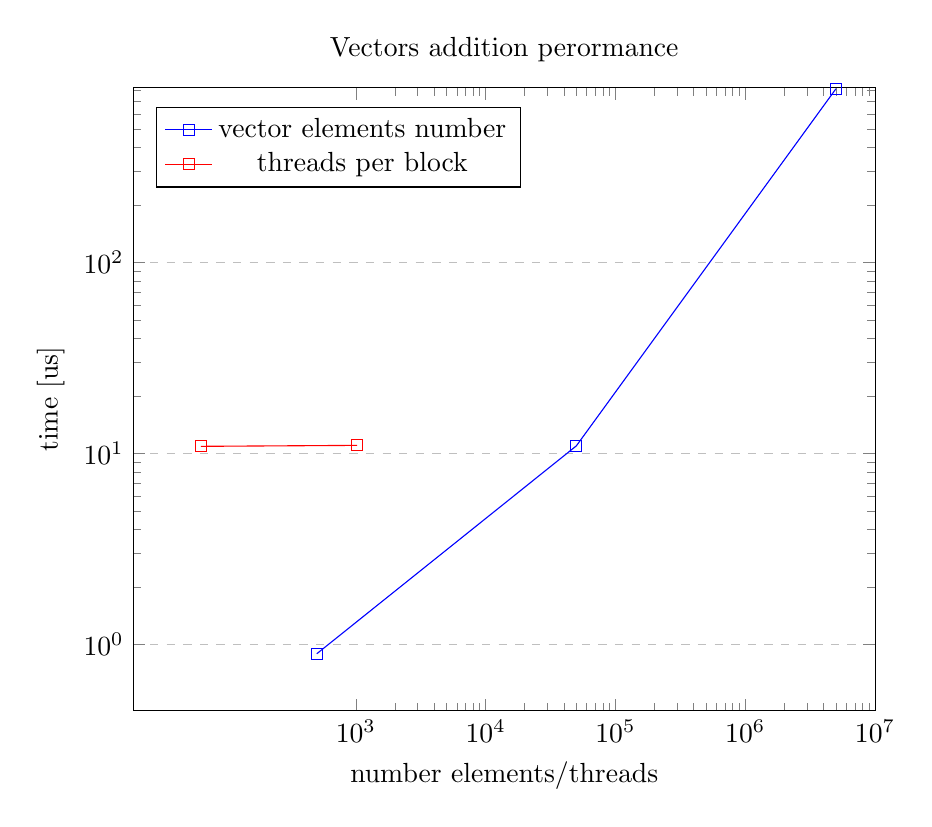
\begin{tikzpicture}
\begin{axis}[
	ymode=log,
	xmode=log,
    title={Vectors addition perormance},
    xlabel={number elements/threads},
    ylabel={time [us]},
    xmin=0, xmax=10000000,
    ymin=0, ymax=820,
    xtick={0,1000,10000,100000,1000000,10000000},
    ytick={1,10,100,1000},
    legend pos=north west,
    ymajorgrids=true,
    grid style=dashed,
]
 
\addplot[
    color=blue,
    mark=square,
    ]
    coordinates {
    (500,0.896)(50000,10.976)(5000000,811.21)
    };
    \addlegendentry{vector elements number}
\addplot[
    color=red,
    mark=square,
    ]
    coordinates {
    (64,10.912)(1024,11.040)
    };
    \addlegendentry{threads per block}
 
\end{axis}
\end{tikzpicture}

A huge difference can be seen when changing data size by two orders of magnitude, whereas changing number of threads from very small (64) to very big (1024) does not result in any major change in terms of time performance.


\subsection{Data transfer time comparison} \label{data_transfer}

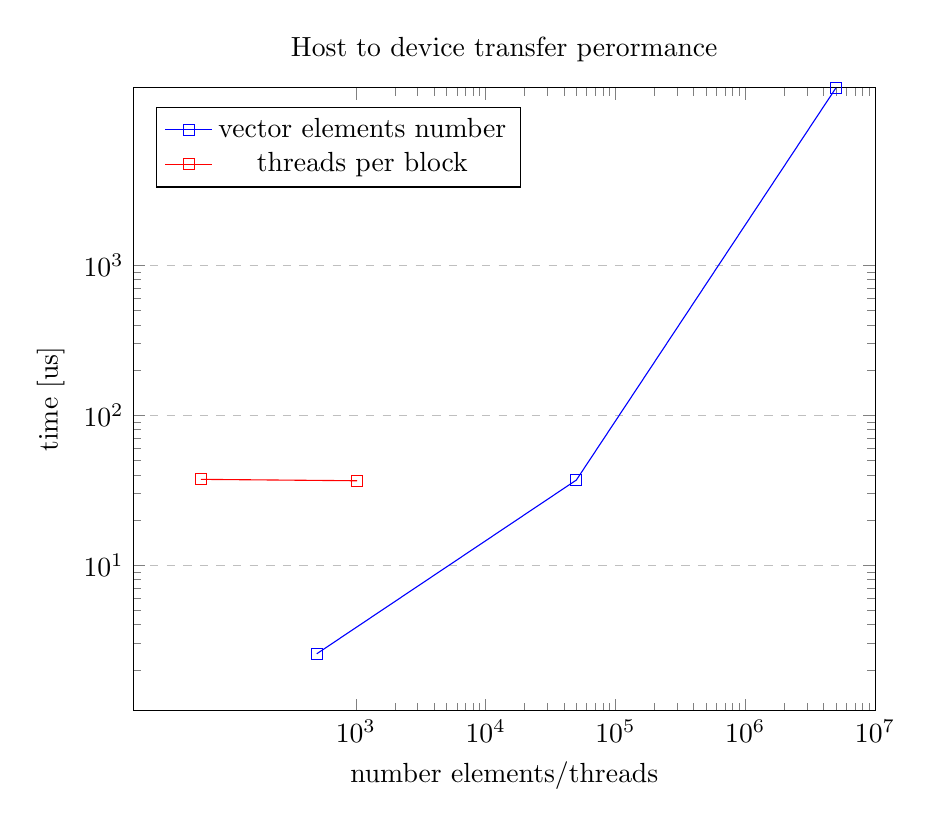
\begin{tikzpicture}
\begin{axis}[
	ymode=log,
	xmode=log,
    title={Host to device transfer perormance},
    xlabel={number elements/threads},
    ylabel={time [us]},
    xmin=0, xmax=10000000,
    ymin=0, ymax=15236,
    xtick={0,1000,10000,100000,1000000,10000000},
    ytick={1,10,100,1000},
    legend pos=north west,
    ymajorgrids=true,
    grid style=dashed,
]
 
\addplot[
    color=blue,
    mark=square,
    ]
    coordinates {
    (500,2.5600)(50000,36.928)(5000000,15236)
    };
    \addlegendentry{vector elements number}
\addplot[
    color=red,
    mark=square,
    ]
    coordinates {
    (64,37.313)(1024,36.513)
    };
    \addlegendentry{threads per block}
 
\end{axis}
\end{tikzpicture}


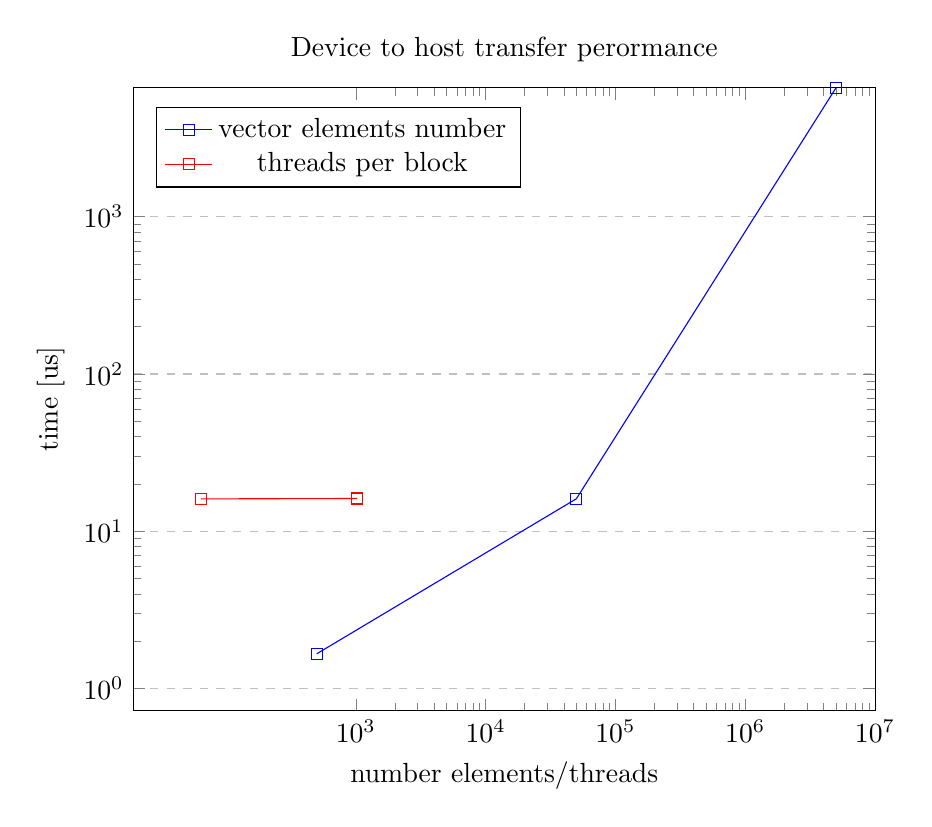
\begin{tikzpicture}
\begin{axis}[
	ymode=log,
	xmode=log,
    title={Device to host transfer perormance},
    xlabel={number elements/threads},
    ylabel={time [us]},
    xmin=0, xmax=10000000,
    ymin=0, ymax=6587,
    xtick={0,1000,10000,100000,1000000,10000000},
    ytick={1,10,100,1000},
    legend pos=north west,
    ymajorgrids=true,
    grid style=dashed,
]
 
\addplot[
    color=blue,
    mark=square,
    ]
    coordinates {
    (500,1.6640)(50000,16.096)(5000000,6587)
    };
    \addlegendentry{vector elements number}
\addplot[
    color=red,
    mark=square,
    ]
    coordinates {
    (64,16.064)(1024,16.160)
    };
    \addlegendentry{threads per block}
 
\end{axis}
\end{tikzpicture}

Although transfer times differ for copying from and to the device, plots look like more or less the same for both operations.

Generally, for all actions on which experiments were conucted the time change is smaller for low figures (for change from 500 to 50 000 - two orders of magnitude - time increased by c. one order of magnitude) and bigger for high figures (for change from 50 000 to 5 000 000 - also two orders - we gained c. two orders of magnitude). It indicates, that using GPU with large number of data transfered at the same time can be less beneficial than granulating this data into subsets and processing them in small portions in GPU. That is why we should try to form our computations in group of smaller calculations, but not too small to aviod too fequent and unnecessary data copying between host and device.

\end{document}